\chapter{Methodology}
\label{chap:methodology}

This chapter describes the full methodology of the thesis. It is organized into two coupled parts. The first
(\Crefrange{sec:meth_dataset}{sec:meth_validation}) defines the physics-informed multi-artifact corruption protocol
that produces the paired (corrupted, ground-truth) examples used for training and evaluation. The second
(\Crefrange{sec:meth_arch}{sec:meth_training}) defines the cascaded encoder--decoder architectures that are trained on those examples, including the alternative-filter input scheme that distinguishes the second stage from a plain image-domain
refinement. The chapter ends with the implementation details and the modeling simplifications that are inherited from
both parts (\Cref{sec:meth_implementation}).

\section{Overview and Design Rationale}
\label{sec:meth_overview}
\label{chap:corruption}%

A core premise of this thesis is that the learned restoration models \gls{ct} must be trained in corruption distributions that reflect the compound nature of clinical acquisition, rather than in a isolated degradation. Clinical CT images
rarely carry only one defect: a post-operative chest scan acquired at reduced dose may simultaneously exhibit
Poisson-limited quantum noise, respiratory motion blur, ring artifacts from a miscalibrated detector element, and metal
streaks from an implant or surgical clip. Comprehensive reviews of the types of CT artifacts in clinical practice note that these degradations arise from distinct physical mechanisms and co-exist routinely in the same
slice~\cite{Boas2012, Gjesteby2016}. Yet, most learned-denoising literature evaluates a network against a single artifact
type in isolation, most often simulated Poisson noise at a fixed dose level.

The protocol presented here is governed by three design choices.

\textbf{(1)~Injection in the sinogram domain.} All physical artifacts considered in this work originate in the acquisition chain rather than in the reconstructed image. Respiratory motion induces projection inconsistencies by shifting the object during acquisition~\cite{LuMackie2002, Mao2007}; ring artifacts arise from detector-specific gain or offset errors~\cite{Sijbers2004, Prell2009}; and metal streaks result from photon starvation along rays passing through highly attenuating implants, which are subsequently spread by the \gls{fbp} ramp filter into the characteristic starburst pattern~\cite{Gjesteby2016}. Injecting these effects directly in the image domain, for example by applying motion blur to a reconstructed slice or inserting an artificial high-intensity object, cannot reproduce their reconstruction-mediated propagation. Sinogram-domain injection is therefore the physically consistent way to model how these artifacts arise and interact with \gls{fbp}~\cite{Mao2007}.

\textbf{(2)~Compound, independently gated mixture.} Rather than training a separate specialist model for each artifact type, we expose a single network to all combinations of corruption. Each of the three physical artifacts is activated independently with a per-sample Bernoulli probability, so that the training distribution contains examples with none, any subset, or all three artifacts simultaneously. Because Poisson noise is already present in every \mbox{LoDoPaB} sinogram (see \Cref{sec:meth_poisson}), every sample is noisy; the physical artifacts are additional overlaid corruptions. This design reflects the clinical setting, in which low-dose noise is ubiquitous whereas specific physical artifacts occur only in some cases.

\textbf{(3)~Physical scale preservation.} \mbox{LoDoPaB} sinograms are stored in post-log form and normalized by $\mu_{\max}=\SI{81.36}{\per\metre}$~\cite{Leuschner2021}, so their values lie nominally in $[0,1]$. All artifacts in the proposed protocol are applied in this $\mu_{\max}$-normalized scale, and the corrupted sinogram is clipped back to $[0,1]$ before reconstruction. No additional $z$-score normalization is introduced, preserving compatibility with the official \mbox{LoDoPaB} baselines~\cite{Leuschner2021, Kiss2024}.

\Cref{fig:meth_pipeline} summarizes the full pipeline. Starting from a \mbox{LoDoPaB} sinogram $\mathbf{s}$ (which already contains simulated low-dose Poisson noise at $N_0=4096$), the three physical corruptions are applied sequentially under their respective Bernoulli gates, after which the result is clipped and reconstructed by \gls{fbp}. This yields a corrupted image $\tilde{\mathbf{x}}=\mathcal{R}^{-1}\tilde{\mathbf{s}}$, which serves as the network input. The ground-truth image $\mathbf{x}$ provided by \mbox{LoDoPaB} is used as the supervision target.
\begin{figure}[!htb]
    \centering
    \begin{tikzpicture}[
        node distance=6mm and 10mm,
        every node/.style={font=\small},
        block/.style={
            rectangle, rounded corners=3pt, draw, very thick,
            minimum width=72mm, minimum height=11mm,
            align=center, fill=blue!5
        },
        gate/.style={
            rectangle, rounded corners=2pt, draw, dashed,
            minimum width=32mm, minimum height=8mm,
            align=center, fill=gray!10, font=\footnotesize
        },
        endblock/.style={block, fill=green!8},
        arrow/.style={->, >=stealth, thick},
        gatearrow/.style={->, >=stealth, dashed}
    ]
        \node[block] (input)
            {\mbox{LoDoPaB} sinogram $\mathbf{s}$ (noisy)\\
             \footnotesize post-log, $\mu_{\max}$-normalized; inherits $N_0{=}4096$ Poisson noise};
        \node[block, below=of input] (motion)
            {Motion shift $\mathcal{T}_\mathrm{mot}$\\
             \footnotesize sinusoidal detector-axis shift};
        \node[block, below=of motion] (ring)
            {Ring offset $\mathcal{T}_\mathrm{ring}$\\
             \footnotesize per-column additive offset};
        \node[block, below=of ring] (metal)
            {Metal injection $\mathcal{T}_\mathrm{met}$\\
             \footnotesize forward-projected mask + photon-starvation clip};
        \node[block, below=of metal] (clip)
            {Clip $\tilde{\mathbf{s}}$ to $[0,1]$};
        \node[block, below=of clip] (fbp)
            {Filtered back-projection $\mathcal{R}^{-1}$};
        \node[endblock, below=of fbp] (out)
            {Network input $\tilde{\mathbf{x}}$};

        \node[gate, right=of motion] (gmot)  {$b_1\sim\mathrm{Bern}(0.5)$};
        \node[gate, right=of ring]   (gring) {$b_2\sim\mathrm{Bern}(0.5)$};
        \node[gate, right=of metal]  (gmet)  {$b_3\sim\mathrm{Bern}(0.3)$};

        \draw[arrow] (input)  -- (motion);
        \draw[arrow] (motion) -- (ring);
        \draw[arrow] (ring)   -- (metal);
        \draw[arrow] (metal)  -- (clip);
        \draw[arrow] (clip)   -- (fbp);
        \draw[arrow] (fbp)    -- (out);

        \draw[gatearrow] (gmot)  -- (motion);
        \draw[gatearrow] (gring) -- (ring);
        \draw[gatearrow] (gmet)  -- (metal);
    \end{tikzpicture}
    \caption[Physics-informed multi-artifact injection pipeline.]{%
        Physics-informed multi-artifact injection pipeline. \mbox{LoDoPaB} sinograms (post-log,
        $\mu_{\max}$-normalized, already containing low-dose Poisson noise at $N_0{=}4096$) pass through three
        sinogram-domain corruption stages, each gated by an independent Bernoulli draw. The corrupted sinogram
        $\tilde{\mathbf{s}}$ is clipped to $[0,1]$ and reconstructed via \gls{fbp} to produce the network input $\tilde{\mathbf{x}}$.}
    \label{fig:meth_pipeline}
\end{figure}

\section{Dataset and Geometry}
\label{sec:meth_dataset}

The base dataset used in this thesis is \mbox{LoDoPaB-CT}~\cite{Leuschner2021}, a public low-dose benchmark derived from the \emph{LIDC/IDRI} thoracic CT collection. It provides \num{42895} paired $(\text{noisy sinogram},\,\text{ground-truth image})$ samples together with a deterministic train/validation/test split. The acquisition and reconstruction geometry adopted throughout this thesis, identical to that of Leuschner et al.~\cite{Leuschner2021}, is summarized in~\Cref{tab:meth_geometry}.

\begin{table}[!htb]
    \centering
    \caption[LoDoPaB-CT parallel-beam geometry used in this thesis.]{%
        \mbox{LoDoPaB-CT} parallel-beam geometry used in this thesis~\cite{Leuschner2021}. Sinograms and images are stored in $\mu_{\max}$-normalized form, so that values lie nominally in $[0,1]$; multiplication by $\mu_{\max}$ recovers physical linear attenuation coefficients.}
    \label{tab:meth_geometry}
    \begin{tabular}{lll}
        \toprule
        Parameter                           & Symbol         & Value \\
        \midrule
        Projection angles                   & $N_\theta$     & $1000$ uniformly in $[0,\pi)$ \\
        Detector elements                   & $N_d$          & $513$ \\
        Reconstruction grid                 & $H \times W$   & $362 \times 362$ \\
        Physical image domain               & $L \times L$   & $\SI{26}{\centi\metre} \times \SI{26}{\centi\metre}$ \\
        Detector pitch                      & $\Delta_d$     & $L\sqrt{2}/N_d \approx \SI{0.72}{\milli\metre}$ \\
        Attenuation normalization           & $\mu_{\max}$   & $\SI{81.36}{\per\metre}$ \\
        Incident photon count               & $N_0$          & $4096$ per detector pixel \\
        Display window                      & $[a,b]$        & $[0,\,0.45]$ ($\mu_{\max}$-normalized) \\
        \bottomrule
    \end{tabular}
\end{table}

Two points should be noted before defining the artifact models. First, the \mbox{LoDoPaB} ground-truth images are cropped to a central \(362 \times 362\) region as part of the original dataset construction~\cite{Leuschner2021}. All images and experiments in this thesis follow that convention. Second, the base sinograms already contain simulated low-dose Poisson noise corresponding to \(N_0 = 4096\) incident photons per detector pixel~\cite{Leuschner2021}. Our protocol therefore does not re-simulate quantum noise, but instead overlays the three additional physical artifacts on top of the provided noisy measurements.

\section{Poisson Noise: Inherited from LoDoPaB}
\label{sec:meth_poisson}

The Beer--Lambert law relates the incident and transmitted photon counts along a ray passing through a slice with attenuation field $\mu(\mathbf{r})$,
\begin{equation}
    I(\ell) \;=\; I_0 \exp\!\left(-\int_{\ell}\mu(\mathbf{r})\,\mathrm{d}\mathbf{r}\right),
    \label{eq:meth_beer_lambert}
\end{equation}
and, for photon-counting detectors, the measured count follows a Poisson distribution,
\begin{equation}
    N \;\sim\; \mathrm{Poisson}\!\big(I_0 \exp(-s)\big), \qquad
    s \;=\; \int_{\ell}\mu(\mathbf{r})\,\mathrm{d}\mathbf{r}.
    \label{eq:meth_poisson}
\end{equation}
\mbox{LoDoPaB} simulates this measurement process at an incident flux of $N_0 = 4096$ photons per detector pixel~\cite{Leuschner2021}. The stored observation is the post-log, $\mu_{\max}$-normalized quantity
\begin{equation}
    \tilde{s}_{\mathrm{LD}} \;=\; -\frac{1}{\mu_{\max}}\,\ln\!\left(\tilde{N}/N_0\right).
    \label{eq:meth_post_log}
\end{equation}
Because this Poisson simulation is performed once during dataset construction and the resulting observations are fixed thereafter, the noise realization is identical across all training runs. Our corruption protocol therefore takes~\eqref{eq:meth_post_log} as its input and adds the three physical artifacts described in the following sections. This choice is deliberate: it preserves direct comparability with the official benchmark setting \mbox{LoDoPaB}~\cite{Leuschner2021, Kiss2024}, whose baselines are evaluated on the same underlying noisy observations.

\section{Motion Artifact}
\label{sec:meth_motion}

\subsection{Physical model}

In parallel-beam CT, a rigid translation of the patient by $(\Delta x, \Delta y)$ at projection angle $\theta$ produces a shift of the sinogram along the detector coordinate $t$ by an angle-dependent amount,
\begin{equation}
    t \;\longrightarrow\; t - \Delta x\cos\theta - \Delta y\sin\theta.
    \label{eq:meth_motion_shift}
\end{equation}
This relation follows directly from the geometry of the Radon transform: a point $(x_0, y_0)$ in image space traces a sinusoidal trajectory in the $(\theta,t)$ sinogram, and a rigid translation shifts that trajectory by the same trigonometric expression. For quasi-periodic respiratory motion, the resulting displacement along the detector axis can be approximated by a sinusoidal function,
\begin{equation}
    \delta t(\theta) \;=\; A \,\sin\!\left(2\pi f\,\theta / N_\theta + \varphi\right),
    \label{eq:meth_motion_periodic}
\end{equation}
where $A$ denotes the peak displacement in detector bins, $f$ is the number of respiratory cycles occurring during the scan, and $\varphi$ is a random initial phase. In our implementation, \eqref{eq:meth_motion_periodic} is applied to each projection row by linear interpolation using \texttt{scipy.ndimage.shift}, with \texttt{mode='nearest'} boundary handling to avoid the non-physical wrap-around artifacts that would arise under \texttt{mode='wrap'}.

\subsection{Parameter choices}

\mbox{LoDoPaB}'s detector pitch is $\Delta_d \approx \SI{0.72}{\milli\metre}$, so a displacement of 10--20 detector bins corresponds to approximately 7--14\,mm of motion along the detector axis. This range is consistent with moderate respiratory motion amplitudes reported for thoracic and abdominal imaging~\cite{Lu2005}. The number of breathing cycles per scan is sampled uniformly from $[0.5, 1.5]$, which produces smooth, coherent projection inconsistencies over the angular range of a scan. In preliminary experiments, smaller amplitudes were often visually masked by the existing Poisson noise floor, whereas substantially higher oscillation frequencies tended to produce sharper streak-like inconsistencies rather than the blurring and double-contour artifacts targeted here.

\begin{table}[!htb]
    \centering
    \caption[Parameters of the motion artifact model.]{%
        Sampling ranges for the motion artifact model. For each enabled sample, $(A, f, \varphi)$ are drawn independently and uniformly from the ranges listed below, with $\varphi \sim \mathcal{U}[0,2\pi)$.}
    \label{tab:meth_motion_params}
    \begin{tabular}{llll}
        \toprule
        Parameter                & Symbol & Range & Physical interpretation \\
        \midrule
        Peak detector shift      & $A$            & $[10,20]$ bins & approximately $7$--$14\,\text{mm}$ motion \\
        Breathing cycles / scan  & $f$            & $[0.5,1.5]$    & quasi-periodic respiration \\
        Initial phase            & $\varphi$      & $[0,2\pi)$     & random scan start phase \\
        Activation probability   & $p_\text{mot}$ & $0.5$          & applied to half of all samples \\
        \bottomrule
    \end{tabular}
\end{table}

\section{Ring Artifact}
\label{sec:meth_ring}

\subsection{Physical model}

Ring artifacts arise when individual detector elements exhibit persistent calibration or sensitivity errors. Because each projection angle is measured by the same detector channels, such errors appear as column-constant stripes in the $(\theta,t)$ sinogram; after \gls{fbp}, these stripes back-project into concentric rings centered on the axis of rotation~\cite{Sijbers2004, Prell2009}. Consider a detector element with multiplicative gain error $g_c$, so that the observed photon count satisfies $\tilde{N}_{\text{obs}} = g_c \tilde{N}_{\text{true}}$. Propagating this error through the LoDoPaB post-log normalization in \eqref{eq:meth_post_log} gives
\begin{equation}
    s_{\text{obs}}(\theta, t_c)
    \;=\; -\frac{1}{\mu_{\max}}\ln\!\left(\frac{g_c \tilde{N}_{\text{true}}}{N_0}\right)
    \;=\; s_{\text{true}}(\theta, t_c) + c_c,
    \qquad
    c_c = -\frac{\ln g_c}{\mu_{\max}}.
    \label{eq:meth_ring_derivation}
\end{equation}
A detector gain error therefore corresponds to an additive offset that is constant across the projection angle in the post-log sinogram. Our corruption model applies this additive perturbation to a sparse random subset $\mathcal{C} \subset \{1,\dots,N_d\}$ of detector columns:
\begin{equation}
    \tilde{s}(\theta, t_c) \;=\; s(\theta, t_c) + c_c,
    \qquad
    c_c \;=\; -\frac{\ln g_c}{\mu_{\max}},
    \qquad
    c \in \mathcal{C}.
    \label{eq:meth_ring}
\end{equation}
Rather than sampling the additive offset $c_c$ directly, we first sample the underlying physical gain $g_c$ and derive $c_c$ from \eqref{eq:meth_ring_derivation}. This ensures that every injected offset corresponds to an interpretable detector state and avoids scale mismatches that could arise if $c_c$ were chosen independently of $\mu_{\max}$. Specifically, we sample $g_c \sim \mathcal{U}[g_{\text{lo}}, g_{\text{hi}}]$ with $0 < g_{\text{lo}} < g_{\text{hi}} < 1$, corresponding to an under-responsive detector element and therefore a bright ring with $c_c > 0$. With probability $\tfrac{1}{2}$, we replace $g_c$ by $1/g_c$ to model an over-responsive element, which produces a dark ring with $c_c < 0$.

\subsection{Parameter choices}

The number of affected detector columns is drawn uniformly from $\{1,\dots,5\}$ out of $N_d=513$, so that ring artifacts arise from a sparse subset of defective elements rather than from widespread detector failure. The gain factor for each affected column is sampled as $g_c \sim \mathcal{U}[0.5,\,0.95]$ or, with probability $\tfrac12$, replaced by its reciprocal to model an over-sensitive detector element. This range spans calibration errors from mild drift (approximately $5\,\%$) to severe response deviation (approximately $50\,\%$), producing both bright and dark rings of varying visibility. Through \eqref{eq:meth_ring_derivation} with $\mu_{\max}=\SI{81.36}{\per\metre}$, these gains correspond to additive post-log offsets of magnitude $|c_c| \in [6.3\times10^{-4},\,8.5\times10^{-3}]$. These values were selected to generate clearly visible but still clinically plausible ring artifacts, consistent with the detector non-uniformity mechanisms described in prior work~\cite{Sijbers2004, Prell2009}.

\begin{table}[!htb]
    \centering
    \caption[Parameters of the ring artifact model.]{%
        Sampling ranges for the ring artifact model. The gain $g_c$ is sampled from the stated range and, with probability $\tfrac12$, replaced by $1/g_c$ to model an over-sensitive detector element. The additive offset $c_c$ is then derived via $c_c=-\ln g_c/\mu_{\max}$.}
    \label{tab:meth_ring_params}
    \small
    \setlength{\tabcolsep}{4pt}
    \begin{tabular}{@{}l l l p{0.32\textwidth}@{}}
        \toprule
        Parameter                    & Symbol                & Range                              & Physical interpretation \\
        \midrule
        Number of affected columns   & $|\mathcal{C}|$       & $\{1,\dots,5\}$                    & sparse detector faults \\
        Detector gain factor         & $g_c$                 & $[0.5,\,0.95]$                     & approximately 5--50\,\% calibration error \\
        Implied additive offset      & $|c_c|$               & $[6.3\times10^{-4},\,8.5\times10^{-3}]$ & $\mu_{\max}$-normalized units \\
        Activation probability       & $p_\text{ring}$       & $0.5$                              & applied to half of all samples \\
        \bottomrule
    \end{tabular}
\end{table}

\section{Metal Artifact}
\label{sec:meth_metal}

\subsection{Physical model}

The metal-artifact model is the most physically involved of the three corruption processes and is constructed from three standard components: (i)~insertion of a dense implant mask in the image domain; (ii)~forward projection through the LoDoPaB parallel-beam geometry to obtain the implant-induced line-integral contribution; and (iii)~detector-level photon-starvation clipping. This sequence follows the general structure of metal-artifact simulation and reduction methods in the CT literature~\cite{Gjesteby2016, Boas2012, ZhangYu2018}.

\paragraph{Image-domain insertion and forward projection.}
Let $\mathbf{m}(x,y)$ denote a binary image-domain mask representing the metal implant, chosen from a simple family of shapes such as disks, ellipses, rectangles or L-shaped brackets to approximate common dental, surgical-clip, and orthopedic cross-sections. Its Radon transform,
\begin{equation}
    s_\mathrm{metal}(\theta,t)
    \;=\; \mathcal{R}\mathbf{m}(\theta,t)
    \;=\; \int_{-\infty}^{\infty}
        \mathbf{m}(t\cos\theta - u\sin\theta,\; t\sin\theta + u\cos\theta)\,\mathrm{d}u,
    \label{eq:meth_metal_fp}
\end{equation}
gives the linear-integral sinogram induced by the implant. Under the monoenergetic Beer--Lambert approximation, insertion of the implant adds this contribution to the tissue line integral along every ray intersecting the metal region, so that the corrupted sinogram becomes
\begin{equation}
    \tilde{s}(\theta,t) \;=\; s(\theta,t) + \alpha\, s_\mathrm{metal}(\theta,t),
    \label{eq:meth_metal_additive}
\end{equation}
where $\alpha$ controls the $\mu_{\max}$-normalized attenuation strength of the inserted metal.

\paragraph{Pre-computation via a library of forward-projected masks.}
Evaluating \eqref{eq:meth_metal_fp} on the fly inside the \texttt{DataLoader} workers is computationally prohibitive, as CPU-based Radon transforms at LoDoPaB resolution require approximately \(0.5\)\,s per sample, while CUDA-based forward projectors do not integrate cleanly with multi-process data loading. We therefore adopt a library-based strategy. A fixed bank of $N_{\text{lib}} = 200$ centered metal masks $\mathbf{m}^{(k)}$, consisting of disks, ellipses, rectangles, and L-shaped brackets with characteristic radii in $[3,12]$\,px (approximately \(2\)--\(9\)\,mm cross-sections), is generated once and forward-projected through the full LoDoPaB geometry on GPU. This yields a corresponding library of centered line-integral sinograms $s_{\mathrm{metal}}^{(k)}$, each normalized to unit peak magnitude. At runtime, an index $k \sim \mathcal{U}\{1,\dots,N_{\text{lib}}\}$ is sampled, and the sinogram contribution of an implant located at an arbitrary position $(x_0,y_0)$ is obtained using the Radon shift identity, which maps image-space translation to a detector-axis shift \(t \mapsto t + x_0\cos\theta + y_0\sin\theta\). In the discrete implementation, this shift is approximated by a per-angle roll along the detector axis.

\paragraph{Photon-starvation clipping.}
Additive line-integral injection alone produces streaks of the correct \emph{shape}, but the \emph{severity} of clinical metal artifacts is driven by a detector-level nonlinearity: rays passing through dense implants may yield near-zero transmitted photon counts, so that the post-log transform becomes unstable and produces strongly amplified streaking~\cite{Gjesteby2016, Boas2012}. We modeled this effect by imposing a one-photon floor on the detector count \emph{after} the additive metal contribution was applied. Writing
\[
    \tilde{N} = N_0 e^{-\tilde{s}\mu_{\max}}
\]
for the implied post-addition photon count, we clip and map back to the stored sinogram scale as
\begin{equation}
    \tilde{N} \;\leftarrow\; \max(\tilde{N},\,1), \qquad
    \tilde{s} \;\leftarrow\; -\frac{1}{\mu_{\max}}\ln(\tilde{N}/N_0).
    \label{eq:meth_metal_starvation}
\end{equation}
This clipping produces the bright and dark saturation streaks that distinguish clinical metal artifacts from a purely additive perturbation along the metal trace. The operation is active only along rays for which the simulated count would otherwise fall below one photon; elsewhere, it reduces to the identity.

\subsection{Parameter choices}

Titanium exhibits strong X-ray attenuation in the diagnostic energy range, so even a small implant cross-section can contribute a substantial additional line integral relative to soft tissue. However, in a simplified monoenergetic model, the resulting artifact strength is typically underestimated because beam hardening and scatter are not explicitly represented~\cite{Boas2012, Gjesteby2016}. We therefore treat the metal scaling parameter $\alpha$ as an effective attenuation factor and sample it from $\alpha \in [0.10, 0.30]$. In combination with the photon-starvation clipping in \eqref{eq:meth_metal_starvation}, this range produces clearly visible streak artifacts of plausible severity while preserving diversity across samples.

Implant positions are sampled uniformly in polar image-domain coordinates, with radius $r \sim \mathcal{U}[0.05, 0.35]\cdot H$ and angle $\theta_0 \sim \mathcal{U}[0, 2\pi)$. The activation probability is set to $p_\mathrm{metal}=0.3$, lower than for motion or ring artifacts, to reflect the case-specific nature of metallic implants and to prevent the severe starvation streaks from dominating the training distribution.

\begin{table}[!htb]
    \centering
    \caption[Parameters of the metal artifact model.]{%
        Sampling ranges for the metal artifact model. The library $\{\mathbf{m}^{(k)}\}$ is a precomputed bank of
        $N_\text{lib}=200$ centered masks; runtime injection consists of library sampling, detector-axis shifting via the
        Radon translation identity, intensity scaling, and photon-starvation clipping according to \eqref{eq:meth_metal_starvation}. The effective metal strength is controlled by $\alpha$, which compensates for artifact-amplifying effects omitted by the monoenergetic model.}
    \label{tab:meth_metal_params}
    \setlength{\tabcolsep}{4pt}
    \small
    \begin{tabular}{@{}l l l l@{}}
        \toprule
        Parameter                    & Symbol              & Range                & Physical interpretation \\
        \midrule
        Number of implants           & $N_\mathrm{impl}$   & $\{1,2\}$            & single or double hardware \\
        Library size                 & $N_\text{lib}$      & $200$                & disks / ellipses / rectangles / L-shapes \\
        Mask radius                  & $r_\mathrm{impl}$   & $[3,12]\,\text{px}$  & approximately $2$--$9\,\text{mm}$ cross-section \\
        Effective metal strength     & $\alpha$            & $[0.10,\,0.30]$      & scaled attenuation contribution \\
        Image-domain radial position & $r/H$               & $[0.05,\,0.35]$      & implant kept inside the FOV \\
        Activation probability       & $p_\mathrm{metal}$  & $0.3$                & case-specific occurrence \\
        Photon-starvation clipping   & ---                 & active               & 1-photon detector floor \\
        \bottomrule
    \end{tabular}
\end{table}

\section{Compound Corruption and Sampling Strategy}
\label{sec:meth_compound}

The three physical artifacts are composed in the order \emph{of motion}$\to$ \emph{ring} $\to$ \emph{metal}, with each transformation activated by an independent Bernoulli gate using the probabilities specified in the preceding sections. Formally, if $\mathcal{T}_\mathrm{mot}$, $\mathcal{T}_\mathrm{ring}$, and $\mathcal{T}_\mathrm{met}$ denote the three sinogram-domain corruption operators, then the final corrupted sinogram is
\begin{equation}
    \tilde{\mathbf{s}} \;=\;
        \mathrm{clip}_{[0,1]}\!\left(
            \mathcal{T}_\mathrm{met}^{b_3}\circ
            \mathcal{T}_\mathrm{ring}^{b_2}\circ
            \mathcal{T}_\mathrm{mot}^{b_1}(\mathbf{s})
        \right),
        \qquad
        b_k \sim \mathrm{Bernoulli}(p_k)\ \text{independent},
    \label{eq:meth_compound}
\end{equation}
where $\mathcal{T}^{0}=\mathrm{id}$ and $\mathcal{T}^{1}=\mathcal{T}$. For $(p_1,p_2,p_3)=(0.5,0.5,0.3)$, approximately $17.5\,\%$ of samples contain no additional physical artifact beyond the inherited Poisson noise, $42.5\,\%$ contain exactly one artifact, $32.5\,\%$ contain two, and $7.5\,\%$ contain all three. The resulting marginal distribution is illustrated in \Cref{fig:meth_frequency}. This distribution is chosen deliberately: it exposes the network to sufficiently many noise-only and single-artifact examples to learn the structure of each individual corruption, while also presenting a substantial fraction of more difficult multi-artifact cases in which restoration must disentangle overlapping degradations~\cite{Boas2012}.
\begin{figure}[!htb]
    \centering
    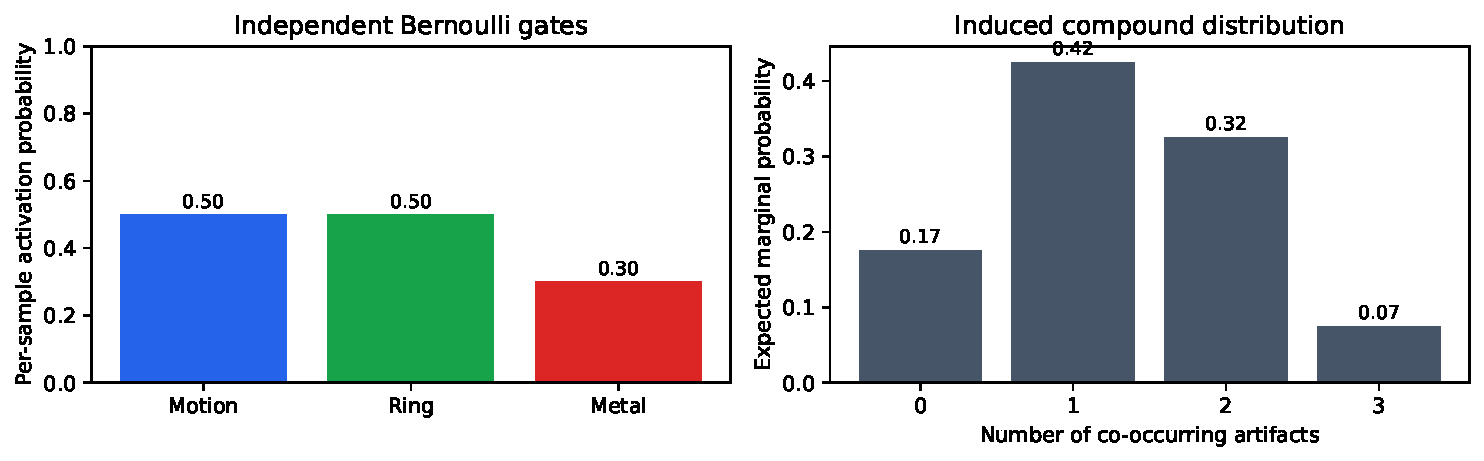
\includegraphics[width=\linewidth]{figures/fig_frequency.pdf}
    \caption[Per-artifact activation and induced compound distribution.]{%
        \textbf{Left:} per-sample Bernoulli activation probabilities for the three physical artifacts. \textbf{Right:}
        induced expected marginal distribution over the number of co-occurring artifacts under the independence assumption.}
    \label{fig:meth_frequency}
\end{figure}
The ordering in \eqref{eq:meth_compound} is chosen to preserve the intended structure of each corruption. Motion is applied first because it operates by interpolation along the detector axis; applying it after ring or metal injection would blur the sharp column-wise perturbations introduced by those artifacts. The final $[0,1]$ clipping step is required because the ring and metal operators can push a small number of bins slightly outside the physically valid range. Clipping removes these unphysical values while preserving consistency with the $\mu_{\max}$-normalized LoDoPaB representation.

\paragraph{Reproducibility of validation and test draws.}
For the training split, artifacts are sampled stochastically, so that each epoch presents a fresh realization of the corruption for every sample. This provides implicit data augmentation over the compound corruption distribution. For the validation and test splits, by contrast, the per-sample random number generator is seeded deterministically as $\mathrm{seed} + \mathrm{idx}$, ensuring that every epoch and every model is evaluated on exactly the same artifact realizations. As a result, comparisons between cascade variants in \Cref{chap:experiments} are not confounded by differences in the corruption draws.

\section{Protocol Validation}
\label{sec:meth_validation}

\Cref{fig:meth_artifact_examples} shows example sinograms and \gls{fbp} reconstructions for a single \mbox{LoDoPaB}
slice under each artifact in isolation and under the compound setting. The qualitative signatures match the physical
expectation: motion produces ghosting and edge-blurring on sharp tissue interfaces; ring artifacts appear as faint
concentric circles inside the patient cross-section; metal produces localized streaks radiating from the implant shadow
location; and the compound case overlays all three in a clinically plausible pattern.
\Cref{fig:meth_severity} complements this with a severity sweep at three operating points per artifact, demonstrating
that the parameter ranges in Tables~\ref{tab:meth_motion_params}--\ref{tab:meth_metal_params} span the
visible-but-not-destructive regime.

\begin{figure}[p]
    \vspace*{0pt}
    \centering
    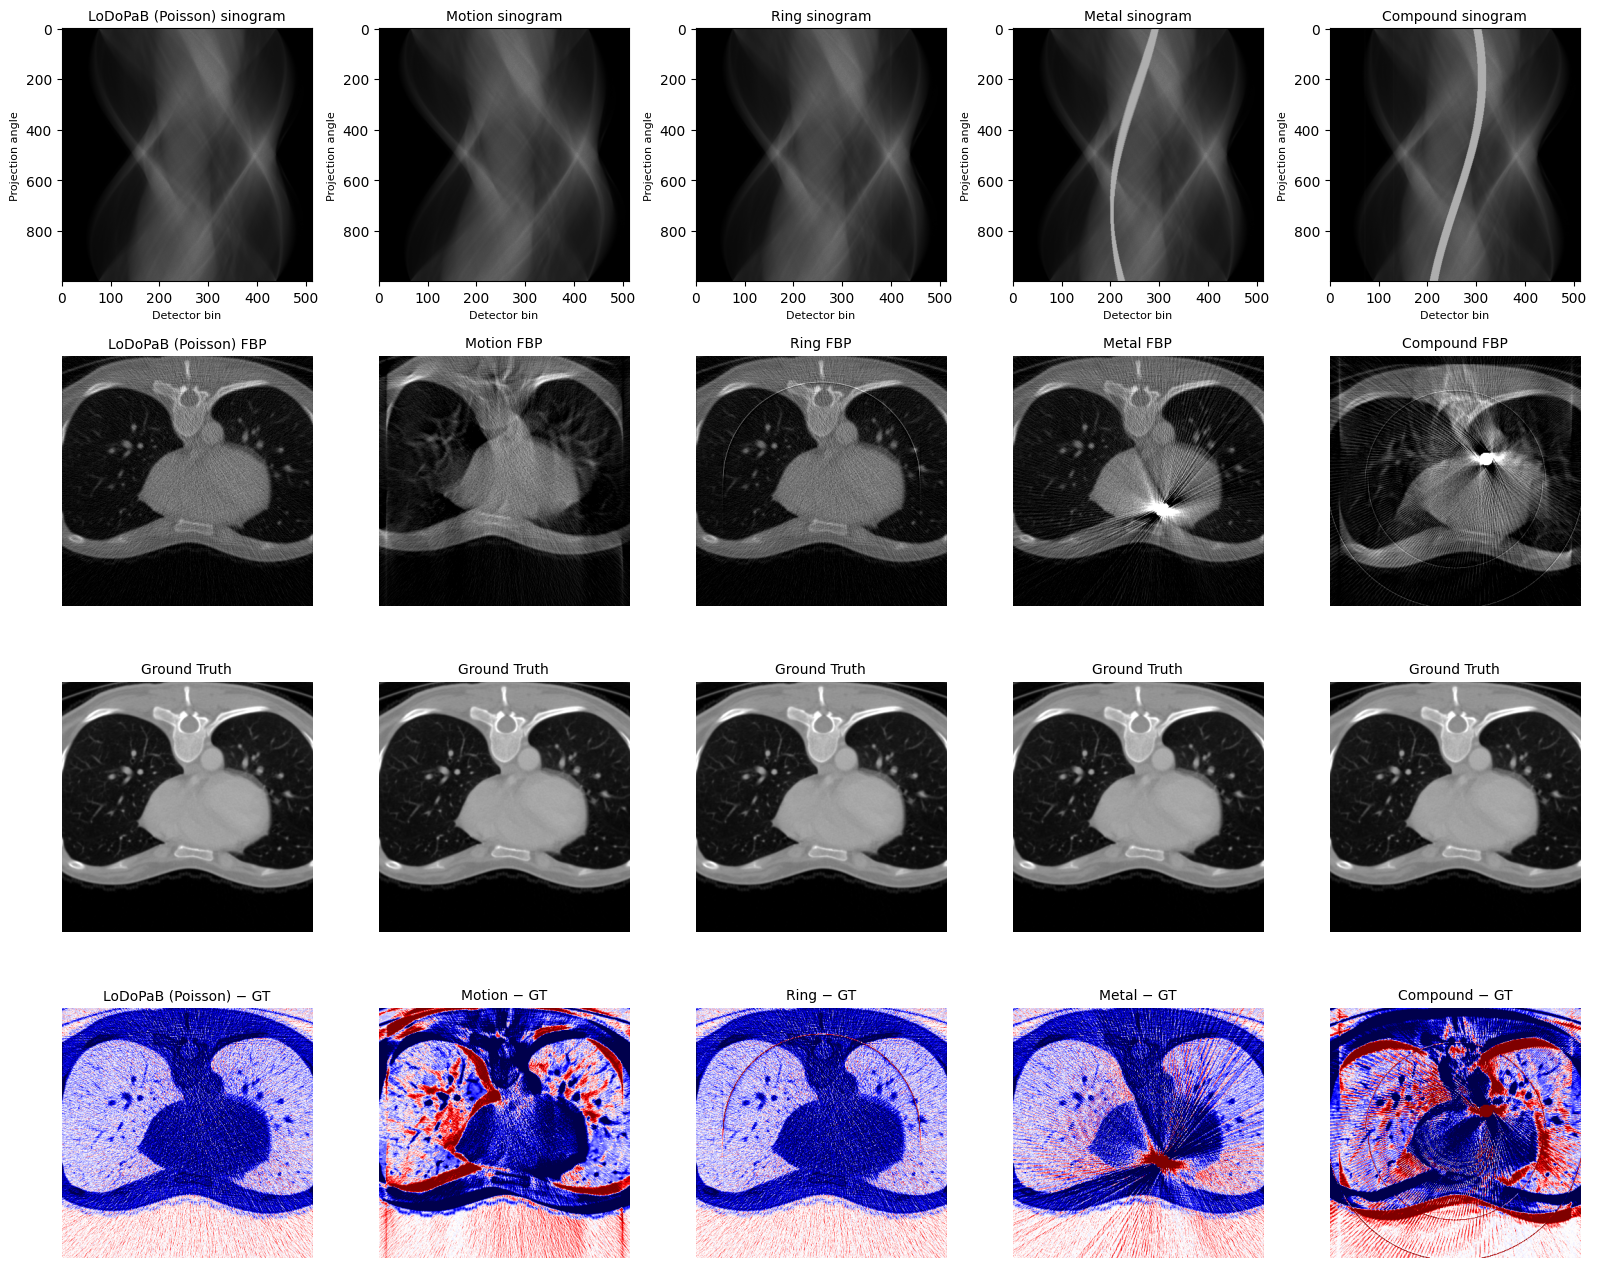
\includegraphics[width=\linewidth]{figures/fig_artifact_examples.png}
    \caption[Qualitative comparison of single and compound artifacts.]{%
        Sinogram (top), \gls{fbp} reconstruction (middle), and signed reconstruction error relative to the ground truth (bottom) for a representative \mbox{LoDoPaB} test slice under each artifact applied in isolation and under the full compound corruption setting. Images are displayed using the \mbox{LoDoPaB} window $[0, 0.45]$~\cite{Leuschner2021}; the error maps use a diverging window of $[-0.1, 0.1]$.}
    \label{fig:meth_artifact_examples}
\end{figure}

\begin{figure}[!htb]
    \centering
    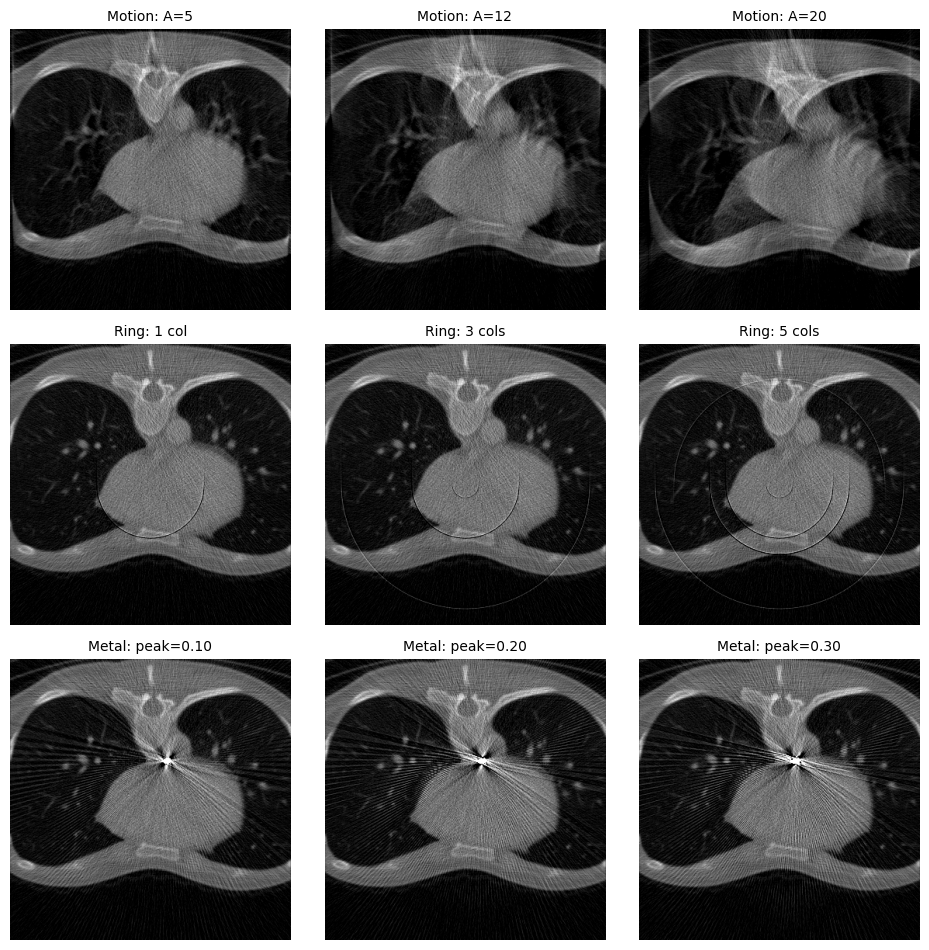
\includegraphics[width=0.95\linewidth]{figures/fig_severity_sweep.png}
    \caption[Severity sweep for each artifact type.]{%
        \gls{fbp} reconstructions shown at three severity levels for each artifact type. The parameter ranges used during training are chosen to span a regime in which the degradations are clearly perceptible while the underlying anatomical structure remains interpretable.}
    \label{fig:meth_severity}
\end{figure}
% \FloatBarrier
%%%%%%%% Cascaded Encoder-- Decoder Architectures
\section{Cascaded Encoder--Decoder Architectures}
\label{sec:meth_arch}
\label{chap:architectures}

This section describes the restoration models evaluated in this thesis. All first stages and all naive-cascade second stages use a plain U-Net backbone~\cite{Ronneberger2015}. Residual-cascade second stages use a ResUNet variant in which every convolutional block is equipped with an intra-block residual shortcut; this architectural change is described in \Cref{subsec:meth_cascade_variants}. Beyond the backbone choice, models differ along three axes: (a)~the number of stages, (b)~the input channels provided to the second stage, and (c)~the way gradients propagate between stages during training.

\subsection{Single-stage U-Net backbone}
\label{subsec:meth_unet}
The backbone is a standard U-Net~\cite{Ronneberger2015} with three downsampling levels and a symmetric upsampling path. Each encoder block consists of two $3{\times}3$ convolutions with GroupNorm and ReLU activations; downsampling is performed by $2{\times}2$ max-pooling. The decoder mirrors the encoder with bilinear upsampling, concatenation-based skip connections at each resolution level, and a final $1{\times}1$ convolution that produces the single-channel output through a sigmoid activation, constraining the prediction to $[0,1]$.

Two capacity configurations are evaluated throughout this work. The \emph{small} variant uses encoder channel widths $[32, 64, 128, 256]$ and has \num{1798113} parameters; the \emph{large} variant uses widths $[64, 128, 256, 512]$ and has \num{7184321} parameters. The resulting single-stage model,
\begin{equation}
    \hat{\mathbf{x}} \;=\; f_{\boldsymbol{\theta}}(\mathbf{y}),
    \label{eq:meth_unet_single}
\end{equation}
is trained end-to-end from scratch and serves both as the standalone baseline and as the first stage of all two-stage cascades introduced in the following.

\subsection{Two-stage cascade: Stage-2 input design}
\label{subsec:meth_cascade_input}

A second stage is introduced to allow further image-domain refinement. In all cascade variants, Stage~1 takes the single-channel Ram--Lak \gls{fbp} reconstruction $\mathbf{y}$ as its input and produces a restored estimate $\hat{\mathbf{x}}_1$. By default, Stage~2 receives only this estimate as a single-channel input:
\begin{equation}
    \mathbf{u}_2 \;=\; \hat{\mathbf{x}}_1.
    \label{eq:meth_default_input}
\end{equation}
This increases processing depth but does not introduce any additional measurement information beyond what is already encoded in $\hat{\mathbf{x}}_1$.

\paragraph{Dual-filter variant.}
One configuration studied in this work augments the Stage~2 input with two additional \gls{fbp} reconstructions computed from the same corrupted sinogram $\tilde{\mathbf{s}}$ using alternative reconstruction filters:
\begin{equation}
    \mathbf{u}_2^{(\mathrm{dual})}
    \;=\; \bigl[\,\hat{\mathbf{x}}_1\;\Vert\;\mathbf{y}^{(\mathrm{Hann})}\;\Vert\;\mathbf{y}^{(\mathrm{SL})}\,\bigr],
    \qquad
    \mathbf{y}^{(h)} \;=\; \mathcal{R}^{-1}_{h}\!\bigl(\tilde{\mathbf{s}}\bigr),
    \label{eq:meth_alt_input}
\end{equation}
where $\mathbf{y}^{(\mathrm{Hann})}$ and $\mathbf{y}^{(\mathrm{SL})}$ denote \gls{fbp} reconstructions produced with the Hann and Shepp--Logan filters, respectively, and $\Vert$ denotes channel-wise concatenation, giving Stage~2 a three-channel input. Different reconstruction filters realize different trade-offs between noise suppression and spatial resolution~\cite{KakSlaney1988}: Ram--Lak preserves sharp detail but amplifies noise, whereas Hann and Shepp--Logan produce smoother images at the cost of reduced high-frequency structure. Providing all three to Stage~2 supplies complementary image-domain information without introducing a learned sinogram-domain component. The resulting cascade is therefore not a dual-domain method~\cite{Wang2020, Zhang2022}, but a multi-input image-domain cascade.

In all variants that do not use the dual-filter extension, Stage~2 receives only $\hat{\mathbf{x}}_1$ (one channel). The dual-filter variant is evaluated only in combination with the residual cascade and is explicitly labelled throughout \Cref{chap:experiments}.
%%─────────────────────────────────────────────────────────
%% Three coupling variants
%%─────────────────────────────────────────────────────────
\subsection{Three coupling variants}
\label{subsec:meth_cascade_variants}

Given the two-stage backbone, three variants are defined by how the parameters
$\{\boldsymbol{\theta}_1, \boldsymbol{\theta}_2\}$ are optimized.

\paragraph{Independent-stage cascade.}
Both stages are trained simultaneously under the cascade loss
$\mathcal{L}^{\mathrm{cascade}}$ of \Cref{eq:meth_loss_cascade_weighted}, but with a
stop-gradient operator applied to $\hat{\mathbf{x}}_{1}$ before it enters Stage~2:
\begin{equation}
    \hat{\mathbf{x}}_{2}
    \;=\; f_{\boldsymbol{\theta}_{2}}\!\bigl(\mathrm{sg}(\mathbf{u}_2)\bigr),
    \label{eq:meth_ind_input}
\end{equation}
where $\mathrm{sg}(\cdot)$ denotes the stop-gradient operator and $\mathbf{u}_2$ is the Stage-2
input defined in \Cref{eq:meth_default_input,eq:meth_alt_input}. Stage~1 is supervised directly
by $\mathcal{L}^{(1)}$; the gradient of $\mathcal{L}^{(2)}$ is blocked at the stage boundary
and does not reach $\boldsymbol{\theta}_1$. Stage~2 is updated only by $\mathcal{L}^{(2)}$.
The two parameter sets are therefore optimized concurrently but with fully decoupled gradient
signals.

\paragraph{End-to-end cascade.}
Both stages are trained jointly under the weighted loss
$\mathcal{L}^{\mathrm{cascade}}$ of \Cref{eq:meth_loss_cascade_weighted},
applied to
\begin{equation}
    \hat{\mathbf{x}}_{2}
    \;=\; f_{\boldsymbol{\theta}_{2}}\!\bigl(\mathbf{u}_2\bigr).
    \label{eq:meth_e2e_input}
\end{equation}
Gradients flow through both stages, allowing earlier-stage features to specialize in service of the
final output. The per-stage weights $(w_{1}, w_{2}) = (0.5,\,0.5)$ in
\Cref{eq:meth_loss_cascade_weighted} mitigate the vanishing-gradient risk of the longer optimization
chain~\cite{He2016}.

\paragraph{Residual cascade.}
Stage~2 is reformulated to predict an additive correction to Stage~1 rather than the clean image directly:
\begin{equation}
    \hat{\mathbf{x}}_{2} \;=\; \hat{\mathbf{x}}_{1}
        \,+\, f_{\boldsymbol{\theta}_{2}}\!\bigl(\mathbf{u}_2\bigr),
    \label{eq:meth_residual}
\end{equation}
where $\mathbf{u}_2$ is either $\hat{\mathbf{x}}_1$ (single-channel default) or $\mathbf{u}_2^{(\mathrm{dual})}$ (\Cref{eq:meth_alt_input}) for the dual-filter variant. Stage~2 in the residual cascade uses a \emph{ResUNet} backbone --- identical in encoder--decoder structure to the U-Net of \Cref{subsec:meth_unet} but with every DoubleConv block replaced by a ResidualDoubleConv block that adds an intra-block shortcut connection and applies its final ReLU to the sum of the convolutional path and the shortcut. The output activation is \texttt{tanh} rather than sigmoid, allowing Stage~2 to predict both positive and negative corrections; the final image is obtained by clamping $\hat{\mathbf{x}}_2$ to $[0,1]$ after the addition in \Cref{eq:meth_residual}.

The residual cascade is trained with the independent-stage protocol ---
both stages trained simultaneously, with the stop-gradient operator applied to
$\hat{\mathbf{x}}_{1}$ so that gradients from $\mathcal{L}^{\mathrm{res}}$ do not reach
$\boldsymbol{\theta}_1$ --- under the three-term loss
$\mathcal{L}^{\mathrm{res}}$ of \Cref{eq:meth_loss_residual}. The residual $\ell^{1}$ term penalizes
the predicted correction directly, while the SSIM and gradient terms supervise the structural and
edge fidelity of the final image.

It should be noted that the residual cascade differs from the naive independent cascade along three dimensions simultaneously: (i)~the Stage~2 output representation changes from a direct image prediction to an additive correction; (ii)~the Stage~2 loss changes from the balanced SSIM\,+\,$\ell^{1}$ objective to the three-term residual loss $\mathcal{L}^{\mathrm{res}}$; and (iii)~the Stage~2 backbone changes from a plain U-Net to a ResUNet with intra-block residual shortcuts. Because no ablation isolates each factor independently, any performance difference observed in \Cref{chap:experiments} reflects the combined effect of all three changes and cannot be attributed to any single design choice alone.


%%─────────────────────────────────────────────────────────
%% Asymmetric-capacity probe
%%─────────────────────────────────────────────────────────
\subsection{Asymmetric-capacity probe}
\label{subsec:meth_asymmetric}

The three coupling variants of \Cref{subsec:meth_cascade_variants} hold stage capacity fixed:
both stages share the same channel widths. This leaves open a separate question about
\emph{capacity allocation}: if Stage~1 is given more parameters, does Stage~2 receive a cleaner
input and therefore converge to a better solution, or does the gain saturate regardless of how
capacity is distributed between stages?

To probe this we define two \emph{asymmetric} cascade configurations that re-allocate the total
parameter budget between the two stages:
\begin{itemize}
    \item \textbf{Large\,$\to$\,small.} Stage~1 uses the large U-Net (channel widths
        $[48,96,192,384]$, ${\approx}4.04$\,M parameters); Stage~2 uses the small ResUNet
        (channel widths $[16,32,64,128]$, ${\approx}0.47$\,M parameters). The hypothesis is
        that a stronger Stage~1 reduces the residual error handed to Stage~2, which Stage~2
        should then find easier to correct even with fewer parameters.
    \item \textbf{Small\,$\to$\,large.} Stage~1 uses the small U-Net (channel widths
        $[16,32,64,128]$, ${\approx}0.45$\,M parameters); Stage~2 uses the large ResUNet
        (channel widths $[48,96,192,384]$, ${\approx}4.24$\,M parameters). This tests the converse:
        whether greater Stage~2 capacity can compensate for a weaker Stage~1 input.
\end{itemize}
Both asymmetric configurations are trained with the independent-stage residual protocol
(\Cref{subsec:meth_cascade_variants}): both stages train simultaneously, with the stop-gradient
operator applied to $\hat{\mathbf{x}}_{1}$ so that Stage~2 is updated only by
$\mathcal{L}^{(2)}$ and Stage~1 only by $\mathcal{L}^{(1)}$. If the cascade gain is primarily
limited by \emph{available residual information} --- that is, by what Stage~1 failed to correct
--- then large\,$\to$\,small should outperform small\,$\to$\,large even though the latter has
more Stage~2 capacity. Conversely, if the gain is limited by Stage~2's representational ability,
the small\,$\to$\,large configuration should close the gap. The experimental outcomes are reported
in \Cref{sec:exp_quantitative}.

\Cref{tab:meth_model_configs} summarizes the backbone, feature widths, input channels, and parameter counts for all model configurations studied in this thesis.

\clearpage
\begin{table}[!ht]
    \centering
    \caption[Architecture and parameter counts for all studied model configurations.]{%
        Architecture and parameter counts for all model configurations. Stage~1 always uses the plain U-Net backbone with sigmoid output. Stage~2 in the naive cascade uses the same plain U-Net; Stage~2 in the residual cascade uses the ResUNet backbone with tanh output. The dual-filter extension adds the Hann and Shepp--Logan \gls{fbp} reconstructions as two extra input channels to Stage~2, increasing its input from 1 to 3 channels.}
    \label{tab:meth_model_configs}
    \setlength{\tabcolsep}{4pt}
    \small
    \begin{tabular}{@{}llllrr@{}}
        \toprule
        Configuration & Stage & Backbone & Features & in\_ch & Params \\
        \midrule
        \multicolumn{6}{l}{\textit{Single-stage baselines}} \\
        U-Net (small)  & Stage~1 & U-Net   & $[32,64,128,256]$  & 1 & \num{1798113} \\
        U-Net (large)  & Stage~1 & U-Net   & $[64,128,256,512]$ & 1 & \num{7184321} \\
        \midrule
        \multicolumn{6}{l}{\textit{Naive cascade — U-Net\,+\,U-Net (sigmoid)}} \\
        Small\,+\,small (detach / e2e)
                       & Stage~1 & U-Net   & $[32,64,128,256]$  & 1 & \num{1798113} \\
                       & Stage~2 & U-Net   & $[32,64,128,256]$  & 1 & \num{1798113} \\
        Large\,+\,large (detach)
                       & Stage~1 & U-Net   & $[48,96,192,384]$  & 1 & \num{4042705} \\
                       & Stage~2 & U-Net   & $[48,96,192,384]$  & 1 & \num{4042705} \\
        \midrule
        \multicolumn{6}{l}{\textit{Residual cascade — U-Net\,+\,ResUNet (tanh)}} \\
        Symmetric small
                       & Stage~1 & U-Net   & $[32,64,128,256]$  & 1 & \num{1798113} \\
                       & Stage~2 & ResUNet & $[32,64,128,256]$  & 1 & \num{1884865} \\
        Symmetric small (dual-filter)
                       & Stage~1 & U-Net   & $[32,64,128,256]$  & 1 & \num{1798113} \\
                       & Stage~2 & ResUNet & $[32,64,128,256]$  & 3 & \num{1885505} \\
        Asym.\ large$\to$small
                       & Stage~1 & U-Net   & $[48,96,192,384]$  & 1 & \num{4042705} \\
                       & Stage~2 & ResUNet & $[16,32,64,128]$   & 1 & \num{472417}  \\
        Asym.\ small$\to$large
                       & Stage~1 & U-Net   & $[16,32,64,128]$   & 1 & \num{450545}  \\
                       & Stage~2 & ResUNet & $[48,96,192,384]$  & 1 & \num{4237345} \\
        \bottomrule
    \end{tabular}
\end{table}

\Cref{fig:meth_cascade_variants} summarizes the data flow and all architectural variants
defined in \Crefrange{subsec:meth_unet}{subsec:meth_asymmetric}.

%% architecture figure
\begin{figure}[!htb]
\centering
%%─────────────────────────────────────────────────────────
%% (a)  Two-stage cascade: data flow
%%─────────────────────────────────────────────────────────
\begin{tikzpicture}[
    every node/.style={font=\footnotesize},
    blk/.style={rectangle, rounded corners=3pt, draw, very thick,
                minimum width=24mm, minimum height=12mm, align=center},
    io/.style={rectangle, rounded corners=2pt, draw,
               minimum width=14mm, minimum height=9mm,
               align=center, fill=gray!8},
    lossnd/.style={circle, draw, fill=yellow!20, minimum size=8mm},
    arr/.style={->, >=Stealth, thick},
    garr/.style={->, >=Stealth, thick, red!60!black, densely dashed},
    larr/.style={->, >=Stealth, gray, thin},
]
    \node[io] (y)    {$\mathbf{y}$\\[-2pt]\tiny Ram--Lak};
    \node[blk, fill=orange!10, right=10mm of y]  (stI)
        {Stage~1\\[-2pt]\tiny U-Net $f_{\theta_1}$};
    \node[io, right=10mm of stI] (x1)   {$\hat{\mathbf{x}}_1$};
    \node[circle, draw, fill=gray!12, minimum size=10mm,
          right=8mm of x1] (cat) {$\Vert$};
    \node[blk, fill=teal!10, right=8mm of cat]   (stII)
        {Stage~2\\[-2pt]\tiny U-Net $f_{\theta_2}$};
    \node[io, right=10mm of stII] (x2)   {$\hat{\mathbf{x}}_2$};
    \node[io, below=14mm of cat] (yalt)
        {$\mathbf{y}^{(\mathrm{Hann})},\mathbf{y}^{(\mathrm{SL})}$\\[-2pt]\tiny dual-filter only};

    %% Loss nodes
    \node[lossnd, below=8mm of x1, font=\tiny] (LI)  {$\mathcal{L}^{(1)}$};
    \node[lossnd, below=8mm of x2, font=\tiny] (LII) {$\mathcal{L}^{(2)}$};

    \draw[arr]  (y)    -- (stI);
    \draw[arr]  (stI)  -- (x1);
    \draw[arr]  (x1)   -- (cat);
    \draw[arr]  (yalt) -- (cat);
    \draw[arr]  (cat)  -- (stII);
    \draw[arr]  (stII) -- (x2);
    \draw[larr] (x1.south)  -- (LI);
    \draw[larr] (x2.south)  -- (LII);

    %% Backward gradient arc routed above the main row
    \coordinate (stIItop) at ([yshift=8mm]stII.north);
    \coordinate (stItop)  at ([yshift=8mm]stI.north);
    \draw[garr] (stII.north) -- (stIItop)
        -- node[above, font=\tiny, black, midway]
               {gradient path (variant-dependent; see (b)--(d))}
        (stItop) -- (stI.north);
\end{tikzpicture}

\bigskip
%%─────────────────────────────────────────────────────────
%% (b)(c)(d)  Coupling variants
%%─────────────────────────────────────────────────────────
\noindent
\begin{minipage}[t]{0.30\linewidth}
\centering
\begin{tikzpicture}[
    every node/.style={font=\footnotesize},
    sblk/.style={rectangle, rounded corners=2pt, draw, thick,
                 minimum width=16mm, minimum height=9mm, align=center},
    arr/.style={->, >=Stealth},
    larr/.style={->, >=Stealth, gray, thin},
]
    \node[sblk, fill=orange!10] (sta) {Stage~1};
    \node[sblk, fill=teal!10, right=14mm of sta] (stb) {Stage~2};
    \draw[arr] (sta) -- node[above, font=\tiny]{$\hat{\mathbf{x}}_1$} (stb);
    %% stop-gradient bar
    \path (sta.east) -- (stb.west) coordinate[midway] (sgm);
    \draw[very thick, red!70!black]
        ([yshift=4mm]sgm) -- ([yshift=-4mm]sgm);
    \node[font=\tiny, text=red!70!black, xshift=3mm] at (sgm) {sg};
    %% Loss nodes: each stage has its own
    \node[circle, draw, fill=yellow!20, minimum size=7mm,
          below=7mm of sta, font=\tiny] (La) {$\mathcal{L}^{(1)}$};
    \node[circle, draw, fill=yellow!20, minimum size=7mm,
          below=7mm of stb, font=\tiny] (Lb) {$\mathcal{L}^{(2)}$};
    \draw[larr] (sta.south) -- (La);
    \draw[larr] (stb.south) -- (Lb);
\end{tikzpicture}\\[4pt]
\small\textbf{(b)~Independent}\\[1pt]
{\tiny Both stages train simultaneously.\\ $\mathcal{L}^{(2)}$ gradient blocked (sg);\\ Stage~1 updated by $\mathcal{L}^{(1)}$ only.}
\end{minipage}%
\hfill
\begin{minipage}[t]{0.30\linewidth}
\centering
\begin{tikzpicture}[
    every node/.style={font=\footnotesize},
    sblk/.style={rectangle, rounded corners=2pt, draw, thick,
                 minimum width=16mm, minimum height=9mm, align=center},
    arr/.style={->, >=Stealth},
    garr/.style={->, >=Stealth, red!60!black, densely dashed},
    larr/.style={->, >=Stealth, gray, thin},
]
    \node[sblk, fill=orange!10] (sta) {Stage~1};
    \node[sblk, fill=teal!10, right=14mm of sta] (stb) {Stage~2};
    \draw[arr] (sta) -- node[above, font=\tiny]{$\hat{\mathbf{x}}_1$} (stb);
    %% Loss nodes
    \node[circle, draw, fill=yellow!20, minimum size=7mm,
          below=7mm of sta, font=\tiny] (La) {$\mathcal{L}^{(1)}$};
    \node[circle, draw, fill=yellow!20, minimum size=7mm,
          below=7mm of stb, font=\tiny] (Lb) {$\mathcal{L}^{(2)}$};
    \draw[larr] (sta.south) -- (La);
    \draw[larr] (stb.south) -- (Lb);
    %% Backward gradient arc (above): L^(2) gradient reaches Stage 1
    \coordinate (stbtop) at ([yshift=7mm]stb.north);
    \coordinate (statop) at ([yshift=7mm]sta.north);
    \draw[garr] (stb.north) -- (stbtop)
        -- node[above, font=\tiny, black, midway]{$\nabla$}
        (statop) -- (sta.north);
\end{tikzpicture}\\[4pt]
\small\textbf{(c)~End-to-end}\\[1pt]
{\tiny Both stages trained jointly.\\$\mathcal{L}^{(2)}$ gradient propagates\\back through Stage~1.}
\end{minipage}%
\hfill
\begin{minipage}[t]{0.36\linewidth}
\centering
\begin{tikzpicture}[
    every node/.style={font=\footnotesize},
    sblk/.style={rectangle, rounded corners=2pt, draw, thick,
                 minimum width=15mm, minimum height=9mm, align=center},
    arr/.style={->, >=Stealth},
    larr/.style={->, >=Stealth, gray, thin},
]
    \node[sblk, fill=orange!10] (sta) {Stage~1};
    \node[sblk, fill=teal!10, right=11mm of sta] (stb)
        {Stage~2\\\tiny pred.\ $\hat{\mathbf{r}}$};
    \node[circle, draw, fill=gray!12, minimum size=8mm,
          right=8mm of stb, font=\normalsize] (add) {$+$};
    \draw[arr] (sta) -- node[above, font=\tiny]{$\hat{\mathbf{x}}_1$} (stb);
    \draw[arr] (stb) -- node[above, font=\tiny]{$\hat{\mathbf{r}}$} (add);
    %% shortcut: x̂_1 enters + from above
    \draw[arr] (sta.north) -- ++(0,9mm) -| (add.north);
    %% stop-gradient bar
    \path (sta.east) -- (stb.west) coordinate[midway] (sgm2);
    \draw[very thick, red!70!black]
        ([yshift=4mm]sgm2) -- ([yshift=-4mm]sgm2);
    \node[font=\tiny, text=red!70!black, xshift=3mm] at (sgm2) {sg};
    %% Loss at final output
    \node[circle, draw, fill=yellow!20, minimum size=7mm,
          below=7mm of stb, font=\tiny] (La) {$\mathcal{L}^{(1)}$};
    \node[circle, draw, fill=yellow!20, minimum size=7mm,
          below=7mm of add, font=\tiny] (Lb) {$\mathcal{L}^{(2)}_\mathrm{res}$};
    \draw[larr] (sta.south) -- (La);
    \draw[larr] (add.south) -- (Lb);
\end{tikzpicture}\\[4pt]
\small\textbf{(d)~Residual}\\[1pt]
{\tiny Both stages train simultaneously;\\ Stage~2 predicts correction $\hat{\mathbf{r}}$;\\ $\hat{\mathbf{x}}_2 = \hat{\mathbf{x}}_1 + \hat{\mathbf{r}}$.}
\end{minipage}

\bigskip

%%─────────────────────────────────────────────────────────
%% (e)(f)  Asymmetric capacity
%%─────────────────────────────────────────────────────────
\noindent
\begin{minipage}[t]{0.46\linewidth}
\centering
\begin{tikzpicture}[
    every node/.style={font=\footnotesize},
    arr/.style={->, >=Stealth},
]
    \node[rectangle, rounded corners=2pt, draw, thick,
          fill=orange!20, minimum width=30mm, minimum height=11mm,
          align=center] (sta)
        {Stage~1\\[-2pt]\tiny Large U-Net ($4.04$\,M)};
    \node[rectangle, rounded corners=2pt, draw, thick,
          fill=teal!8, minimum width=20mm, minimum height=11mm,
          align=center, right=12mm of sta] (stb)
        {Stage~2\\[-2pt]\tiny Small ResUNet ($0.47$\,M)};
    \draw[arr] (sta) -- node[above, font=\tiny]{$\hat{\mathbf{x}}_1$} (stb);
\end{tikzpicture}\\[4pt]
\small\textbf{(e)~Large $\to$ Small}
\end{minipage}%
\hfill
\begin{minipage}[t]{0.46\linewidth}
\centering
\begin{tikzpicture}[
    every node/.style={font=\footnotesize},
    arr/.style={->, >=Stealth},
]
    \node[rectangle, rounded corners=2pt, draw, thick,
          fill=orange!8, minimum width=20mm, minimum height=11mm,
          align=center] (sta)
        {Stage~1\\[-2pt]\tiny Small U-Net ($0.45$\,M)};
    \node[rectangle, rounded corners=2pt, draw, thick,
          fill=teal!20, minimum width=30mm, minimum height=11mm,
          align=center, right=12mm of sta] (stb)
        {Stage~2\\[-2pt]\tiny Large ResUNet ($4.24$\,M)};
    \draw[arr] (sta) -- node[above, font=\tiny]{$\hat{\mathbf{x}}_1$} (stb);
\end{tikzpicture}\\[4pt]
\small\textbf{(f)~Small $\to$ Large}
\end{minipage}

\caption[Cascade architecture variants.]{%
    \textbf{(a)}~General two-stage cascade data flow. The corrupted FBP
    reconstruction $\mathbf{y}$ (Ram--Lak filter) feeds Stage~1; its output
    $\hat{\mathbf{x}}_1$ forms the Stage~2 input $\mathbf{u}_2$ (single channel by default;
    three channels $[\hat{\mathbf{x}}_1\,\Vert\,\mathbf{y}^{(\mathrm{Hann})}\,\Vert\,\mathbf{y}^{(\mathrm{SL})}]$
    in the dual-filter variant).
    Loss nodes $\mathcal{L}^{(1)}$ and $\mathcal{L}^{(2)}$ supervise
    each stage output. The dashed red arc marks the backward gradient path,
    which is variant-dependent.
    \textbf{(b)~Independent:} both stages train simultaneously; the
    stop-gradient barrier (sg) blocks the $\mathcal{L}^{(2)}$ gradient from
    reaching Stage~1, which is updated only by $\mathcal{L}^{(1)}$.
    \textbf{(c)~End-to-end:} both stages trained jointly; the
    $\mathcal{L}^{(2)}$ gradient $\nabla$ propagates back through Stage~2
    and continues to update Stage~1.
    \textbf{(d)~Residual:} same stop-gradient protocol as (b); Stage~2
    predicts an additive correction $\hat{\mathbf{r}}$, giving
    $\hat{\mathbf{x}}_2 = \hat{\mathbf{x}}_1 + \hat{\mathbf{r}}$;
    the arc above shows the $\hat{\mathbf{x}}_1$ shortcut.
    \textbf{(e)--(f)}~Asymmetric-capacity configurations; block width is
    proportional to parameter count.}
\label{fig:meth_cascade_variants}
\end{figure}

\FloatBarrier

%%─────────────────────────────────────────────────────────
%% section:Loss function
%%─────────────────────────────────────────────────────────
\section{Loss Functions}
\label{sec:meth_loss}

A pure pixel-wise $\ell^{1}$ loss, although widely used in CT restoration and denoising~\cite{Chen2017, Zhang2017}, was found in preliminary experiments to over-smooth high-frequency anatomical detail under the compound-corruption regime considered here. Conversely, pure \gls{ssim} supervision preserved structure well but allowed slight residual intensity drift in smooth regions. We therefore adopt a mixed loss that combines \gls{ssim} with $\ell^{1}$ and, for the residual cascade, an additional finite-difference gradient term to sharpen edges near metal streaks. To keep notation compact, let $\mathcal{L}_{1}$, $\mathcal{L}_{\mathrm{SSIM}}$, and $\mathcal{L}_{\nabla}$ denote, respectively, the pixel-wise \gls{mae}, the structural-similarity loss \(1-\mathrm{SSIM}\)~\cite{Wang2004}, and a finite-difference image-gradient $\ell^{1}$ loss,
\begin{align}
    \mathcal{L}_{1}(\hat{\mathbf{x}}, \mathbf{x}) &\;=\; \frac{1}{HW}\sum_{j}\bigl|\hat{x}_{j} - x_{j}\bigr|,
    \label{eq:meth_l1_loss}\\
    \mathcal{L}_{\mathrm{SSIM}}(\hat{\mathbf{x}}, \mathbf{x}) &\;=\; 1 - \mathrm{SSIM}(\hat{\mathbf{x}}, \mathbf{x}),
    \label{eq:meth_ssim_loss}\\
    \mathcal{L}_{\nabla}(\hat{\mathbf{x}}, \mathbf{x})
        &\;=\; \frac{1}{HW}\sum_{j}\Bigl(
        |\nabla_{x}\hat{x}_{j}-\nabla_{x}x_{j}|
        + |\nabla_{y}\hat{x}_{j}-\nabla_{y}x_{j}|
        \Bigr).
    \label{eq:meth_grad_loss}
\end{align}
These primitive losses are combined into task-specific objectives that are reused across the cascade variants.

\paragraph{Stage~1 --- balanced SSIM + L1.}
Stage~1 is supervised using an equal-weight combination of \gls{ssim} and pixel-wise \gls{mae},
\begin{equation}
    \mathcal{L}^{(1)}\!\bigl(\hat{\mathbf{x}}_{1}, \mathbf{x}\bigr)
    \;=\; 0.5\,\mathcal{L}_{\mathrm{SSIM}}\!\bigl(\hat{\mathbf{x}}_{1}, \mathbf{x}\bigr)
    \;+\; 0.5\,\mathcal{L}_{1}\!\bigl(\hat{\mathbf{x}}_{1}, \mathbf{x}\bigr).
    \label{eq:meth_loss_stage1}
\end{equation}
The \gls{ssim} term promotes local structural agreement with the reference image, while the $\ell^{1}$ term anchors absolute intensity values and reduces low-frequency drift in smooth regions.

\paragraph{Stage~2 in the naive cascade --- same SSIM + L1.}
In the naive cascade variants, Stage~2 predicts the restored image directly and is trained with the same balanced objective,
\begin{equation}
    \mathcal{L}^{(2)}_{\mathrm{naive}}\!\bigl(\hat{\mathbf{x}}_{2}, \mathbf{x}\bigr)
    \;=\; 0.5\,\mathcal{L}_{\mathrm{SSIM}}\!\bigl(\hat{\mathbf{x}}_{2}, \mathbf{x}\bigr)
    \;+\; 0.5\,\mathcal{L}_{1}\!\bigl(\hat{\mathbf{x}}_{2}, \mathbf{x}\bigr).
    \label{eq:meth_loss_naive_stage2}
\end{equation}
Using the same loss in both stages keeps the comparison between the single-stage baseline and the naive two-stage cascades clean: any performance difference is attributable to architectural design or coupling strategy rather than to a change in the objective.

\paragraph{Stage~2 in the residual cascade --- residual L1 + SSIM + gradient.}
In the residual cascade, Stage~2 predicts an additive correction
\[
    \hat{\mathbf{r}}_{2}
    = f_{\boldsymbol{\theta}_{2}}\!\bigl(\mathbf{u}_2\bigr),
\]
with final output \(\hat{\mathbf{x}}_{2}=\hat{\mathbf{x}}_{1}+\hat{\mathbf{r}}_{2}\). It is trained using a three-term loss that penalises the residual prediction itself, the structural quality of the final image, and the fidelity of edge information,
\begin{equation}
    \mathcal{L}^{(2)}_{\mathrm{res}}
    \;=\; 0.4\,\mathcal{L}_{1}\!\bigl(\hat{\mathbf{r}}_{2}, \mathbf{r}\bigr)
    \;+\; 0.3\,\mathcal{L}_{\mathrm{SSIM}}\!\bigl(\hat{\mathbf{x}}_{2}, \mathbf{x}\bigr)
    \;+\; 0.3\,\mathcal{L}_{\nabla}\!\bigl(\hat{\mathbf{x}}_{2}, \mathbf{x}\bigr),
    \label{eq:meth_loss_residual}
\end{equation}
where \(\mathbf{r}=\mathbf{x}-\hat{\mathbf{x}}_{1}\) denotes the target residual. The gradient term compensates for the soft-edge bias that pure SSIM/\(\ell^{1}\) supervision would otherwise leave near sharp metal-streak boundaries.

\paragraph{Per-stage weighting in cascades.}
Whenever a cascade is trained under a single joint objective, both stage outputs contribute with equal weight,
\begin{equation}
    \mathcal{L}^{\mathrm{cascade}}
    \;=\; 0.5\,\mathcal{L}^{(1)}\!\bigl(\hat{\mathbf{x}}_{1}, \mathbf{x}\bigr)
    \;+\; 0.5\,\mathcal{L}^{(2)}\!\bigl(\hat{\mathbf{x}}_{2}, \mathbf{x}\bigr),
    \label{eq:meth_loss_cascade_weighted}
\end{equation}
where \(\mathcal{L}^{(2)}\) is either \eqref{eq:meth_loss_naive_stage2} or \eqref{eq:meth_loss_residual}. Equal per-stage weights provide explicit supervision to the intermediate output and reduce the risk that Stage~1 receives only weak training signals in the end-to-end setting.

A summary of the losses used by each model variant is given in \Cref{tab:meth_losses}.

\begin{table}[!htb]
    \centering
    \caption[Loss function per cascade variant.]{%
        Loss function used to train each model variant. When a cascade is monitored or optimized jointly, both stages contribute with equal weight \(w_{1}=w_{2}=0.5\). SSIM denotes the structural-similarity loss \(1-\mathrm{SSIM}\)~\cite{Wang2004}, and $\mathcal{L}_{\nabla}$ denotes the finite-difference image-gradient $\ell^{1}$ loss.}
    \label{tab:meth_losses}
    \setlength{\tabcolsep}{4pt}
    \small
    \begin{tabular}{@{}l l@{}}
        \toprule
        Variant & Loss \\
        \midrule
        Stage~1 (single-stage U-Net) &
        $0.5\,\mathcal{L}_{\mathrm{SSIM}}(\hat{\mathbf{x}}_{1},\mathbf{x}) + 0.5\,\mathcal{L}_{1}(\hat{\mathbf{x}}_{1},\mathbf{x})$ \\
        Independent-stage naive cascade (Stage~2) &
        $0.5\,\mathcal{L}_{\mathrm{SSIM}}(\hat{\mathbf{x}}_{2},\mathbf{x}) + 0.5\,\mathcal{L}_{1}(\hat{\mathbf{x}}_{2},\mathbf{x})$ \\
        End-to-end naive cascade &
        $0.5\,\mathcal{L}^{(1)}(\hat{\mathbf{x}}_{1},\mathbf{x}) + 0.5\,\mathcal{L}^{(2)}_{\mathrm{naive}}(\hat{\mathbf{x}}_{2},\mathbf{x})$ \\
        Independent-stage residual cascade &
        $0.4\,\mathcal{L}_{1}(\hat{\mathbf{r}}_{2},\mathbf{r}) + 0.3\,\mathcal{L}_{\mathrm{SSIM}}(\hat{\mathbf{x}}_{2},\mathbf{x}) + 0.3\,\mathcal{L}_{\nabla}(\hat{\mathbf{x}}_{2},\mathbf{x})$ \\
        End-to-end residual cascade &
        $0.5\,\mathcal{L}^{(1)}(\hat{\mathbf{x}}_{1},\mathbf{x}) + 0.5\,\mathcal{L}^{(2)}_{\mathrm{res}}$ \\
        \bottomrule
    \end{tabular}
\end{table}
%%─────────────────────────────────────────────────────────
%% Training Procedure
%%─────────────────────────────────────────────────────────
\section{Training Procedure}
\label{sec:meth_training}

All models are trained on the \mbox{LoDoPaB-CT} \texttt{train} split (\num{35820} slices), with the sinogram-domain corruption pipeline of \Cref{sec:meth_compound} applied on the fly during data loading. Model selection is performed on the \texttt{validation} split (\num{3522} slices), and final quantitative results in \Cref{chap:experiments} are reported on the held-out \texttt{test} split (\num{3553} slices). For the validation and test sets, the corruption process is seeded deterministically on a per-sample basis, so that every model is evaluated on exactly the same artifact realizations. No external data are used at any stage: in particular, we do not use clean-CT pre-training, synthetic pretraining on auxiliary datasets, or out-of-domain medical images.

Optimization is carried out using AdamW with the default momentum parameters $(\beta_{1}, \beta_{2}) = (0.9,\,0.999)$. Unless stated otherwise, the learning rate is fixed at $3\times 10^{-4}$ for all proposed models. The only exception is the RED-CNN baseline, which is trained at $1\times 10^{-4}$ in order to match the original training protocol of Chen et al.~\cite{Chen2017}. The mini-batch size is $4$ slices, chosen to fit the U-Net-based models at resolution $362\times 362$ on a single \gls{gpu}. Each model is trained for up to $150$ epochs with early stopping: training is halted if the validation loss does not improve for $15$ consecutive epochs, and the checkpoint achieving the lowest validation loss is retained for final evaluation.

No augmentation beyond stochastic corruption sampling is applied. In particular, random geometric transforms such as flips or rotations are omitted in order to preserve a fixed image orientation throughout training and evaluation. For visual inspection only, images are displayed using the local viewing convention \texttt{np.flipud(x.T)}, but this is a display transform rather than part of the learning pipeline. The effective augmentation therefore comes entirely from the per-epoch resampling of corruption parameters on the training split, which exposes the network to fresh artifact realizations throughout optimization.

\section{Implementation and Known Simplifications}
\label{sec:meth_implementation}

\paragraph{Implementation.}
The corruption pipeline is implemented in \texttt{utils/lodopab\_dataset.py} and executed on the CPU inside the \texttt{Dataset.\_\_getitem\_\_} method. This design places the additional corruption cost in the \texttt{DataLoader} worker processes rather than in the GPU training loop, so artifact synthesis does not block model execution. The metal artifact component relies on a precomputed library generated once by \texttt{scripts/build\_metal\_library.py} on GPU and stored as a memory-mapped \texttt{.npz} file for efficient reuse at training time. In practice, the combined runtime for motion, ring, and metal corruption is only a few milliseconds per sample, and with eight data-loading workers the total artifact-injection overhead is approximately \SI{20}{\second} per epoch over the \num{35820} training slices. All experiments are implemented in PyTorch and run on a single \gls{gpu}.

\paragraph{Known simplifications.}
The corruption model is intentionally lightweight so that it can be applied online during training at negligible computational cost. To make the resulting scope explicit, we summarize the main modeling simplifications in the following.

\begin{enumerate}
    \item \textbf{Monoenergetic metal model.}
    The additive formulation in \eqref{eq:meth_metal_additive} assumes a monoenergetic acquisition model and therefore does not reproduce the full spectral beam-hardening behavior of polyenergetic CT. As a practical approximation, the missing amplification is absorbed empirically into the sampled metal-strength range $\alpha \in [0.10, 0.30]$, following common simplified practice in \gls{mar} simulation. The photon-starvation clipping term in \eqref{eq:meth_metal_starvation} captures the dominant count-rate nonlinearity, but not the full spectral signature associated with beam hardening. A fully polyenergetic forward simulation would require regenerating the measurement process rather than perturbing the fixed LoDoPaB sinograms, and is therefore left for future work.

    \item \textbf{One-dimensional motion projection.}
    The motion model applies the displacement in \eqref{eq:meth_motion_shift} only along the detector coordinate, effectively reducing in-plane motion to a single projected shift in the sinogram domain. This avoids a more expensive re-projection step while still representing the dominant radial component of respiratory motion that is most relevant for thoracic CT slices. The model therefore captures structured view-dependent inconsistency, but not the full angular coupling of independent two-dimensional translation.

    \item \textbf{Integer-bin metal translation.}
    The library-based metal contribution is shifted using integer detector-bin rolls rather than sub-bin interpolation. This introduces a small discretizations error, but in practice its effect is minor relative to the stochastic variation in sampled metal position and intensity, and is further attenuated by the subsequent photon-starvation clipping stage.
\end{enumerate}

These simplifications do not affect the central comparison in \Cref{chap:experiments}, because all model variants are trained and evaluated under the same seeded corruption distribution. The purpose of the protocol is not to reproduce scanner physics exhaustively, but to provide a controlled and repeatable stress test for comparing restoration architectures under consistent mixed-artifact conditions. More realistic polyenergetic simulation and higher-fidelity motion modeling are discussed as natural extensions in \Cref{chap:conclusion}.
